\documentclass[14pt,a4paper,oneside,final]{extreport}

\newcommand{\pwd}{src/uir.nir}

\def\showannotation{false}

\setlength\paperheight{297mm}
\setlength\paperwidth{210mm}


\usepackage{polyglossia}
\setmainlanguage[numerals=cyrillic]{russian}
\setotherlanguages{english}

\usepackage{xunicode} % some extra unicode support
%\usepackage[utf8x]{inputenc}
\usepackage{xltxtra} % \XeLaTeX macro
\usepackage{fontspec}
\defaultfontfeatures{Ligatures=TeX}

%\setromanfont{Charis SIL}
%\setsansfont{Liberation Sans}
%\setmonofont{PT Mono}
%\setmainfont{Liberation Serif} % this allows to use sans-serif as default font

% \newfontfamily{\cyrillicfont}{Times New Roman}
% \setmainfont[Mapping=tex-text]{Times New Roman}
% \newfontfamily{\cyrillicfonttt}{Courier New}
% \setmonofont{Courier New}

\setmainfont{Linux Libertine O}
\setsansfont{Linux Biolinum O}
\setmonofont[SmallCapsFont={Latin Modern Mono Caps}]{Latin Modern Mono Light}

%нумерация справа и колонтитулы справа вверху
\usepackage{fancyhdr}
\usepackage[left=30mm,right=10mm,top=20mm,bottom=20mm,bindingoffset=0cm]{geometry}%

\usepackage{amsfonts}
\usepackage{amssymb}
\usepackage{amsmath}
\usepackage{amsthm}

\usepackage{calc}
\usepackage{ifthen}
\usepackage{graphicx}
\usepackage{array}
\usepackage{pdfpages}
\usepackage{longtable}
\usepackage{tabu}
\usepackage{indentfirst}
\usepackage[unicode=true]{hyperref}
\usepackage{color}
\usepackage{pgf}

\usepackage{./styles/pstheorems}

% Настройка списков (без лишних вертикальных отступов)
\usepackage{paralist}
\setdefaultenum{1.}{1.}{1.}{1.}
\setdefaultitem{{}--{}}{}{}{}
%\setlength\itemsep{-1em}
\let\itemize\compactitem
\let\enditemize\endcompactitem
\let\enumerate\compactenum
\let\endenumerate\endcompactenum
\let\description\compactdesc
\let\enddescription\endcompactdesc
\pltopsep=\smallskipamount
\plitemsep=0pt
\plparsep=0pt
% Команда для отмены разрыва страниц перед списками
\makeatletter 
\newcommand\mynobreakpar{\par\nobreak\@afterheading} 
\makeatother
%%%%%%

\usepackage[singlelinecheck=false,labelsep=endash]{caption}
\captionsetup[table]{justification=justified}
\captionsetup[figure]{justification=centering}

\usepackage{titlesec}
\titleformat{\chapter}[block]{\centering\normalfont\Large\bfseries}{\thechapter.}{1ex}{}{}
\titlespacing{\chapter}{0pt}{\parskip}{-\parskip}%{0em}{2em}

\titleformat{\section}[block]{\normalfont\large\bfseries}{\thesection.}{1ex}{}{}
\titlespacing{\section}{0pt}{\parskip}{-\parskip}%{0em}{1ex}

\titleformat{\subsection}[block]{\normalfont\normalsize\bfseries}{\thesubsection.}{1ex}{}{}
\titlespacing{\subsection}{0pt}{\parskip}{-\parskip}%{0em}{1ex}

	% paragraph и subparagraph -- в тексте, без отступов
\titleformat{\paragraph}[runin]{\normalfont\normalsize\bfseries}{\theparagraph}{0pt}{}{}
\titlespacing{\paragraph}{0pt}{0em}{0ex}

\titleformat{\subparagraph}[runin]{\normalfont\normalsize\bfseries}{\thesubparagraph}{0pt}{}{}
\titlespacing{\subparagraph}{0pt}{0em}{0ex}


% Своё название для Cписка литературы
\usepackage[title, titletoc]{appendix}
\addto\captionsrussian{% Replace "english" with the language you use
	\renewcommand{\contentsname}%
	{Содержание}%
}

%\renewcommand{\appendixname}{Приложение}% Change "chapter name" for Appendix chapters
%\renewcommand{\cftchapdotsep}{\cftdotsep}

\usepackage{./styles/mathpartir}

\makeatletter
\let\ps@plain\ps@fancy              % Подчиняем первые страницы каждой главы общим правилам
\makeatother
\pagestyle{fancy}
\fancyhf{}
\fancyfoot[C]{\thepage}
\renewcommand{\headrulewidth}{0pt}
\renewcommand{\footrulewidth}{0pt}
\renewcommand{\baselinestretch}{1.5}
\newcommand{\headertext}[1]{\fancyhead[R]{\tiny{#1}}}

%% Список литературы

\makeatletter
\bibliographystyle{ugost2008}     % Оформляем список литературы по ГОСТ 7.1
% (ГОСТ Р 7.0.11-2011, 5.6.7)
\renewcommand{\@biblabel}[1]{#1.}   % Заменяем список литературы с квадратных
% скобок на точку
\makeatother

%\frenchspacing %% изменение расстояние до и после точек в ряде случаев

\renewcommand{\theenumi}{\arabic{enumi}}
\renewcommand{\theenumii}{\arabic{enumii}}
\renewcommand{\theenumiii}{\arabic{enumiii}}
\renewcommand{\theenumiv}{\arabic{enumiv}}

\renewcommand{\labelenumi}{\theenumi.}
\renewcommand{\labelenumii}{\theenumi.\theenumii.}
\renewcommand{\labelenumiii}{\theenumi.\theenumii.\theenumiii.}
\renewcommand{\labelenumiv}{\theenumi.\theenumii.\theenumiii.\theenumiv.}

%\newenvironment{annotation}{\textbf{Аннотация.} \textit}{}
\theoremstyle{plain}
\newtheorem*{annotation}{Аннотация}

\usepackage{listingsutf8}

\renewcommand{\lstlistingname}{Листинг}

\lstset{
  language=[Sharp]C,
  basicstyle=\linespread{0.94}\ttfamily,
  tabsize=2,
  showstringspaces=false,
  columns=flexible,
  numbers=left,
  numberstyle=\normalsize\color{gray},
  breaklines=true,
  breakatwhitespace=true,
  framesep=6pt,
  abovecaptionskip=1em,
  captionpos=b,
  extendedchars=\true,
  inputencoding=utf8,
  xleftmargin=22pt,
  literate={Ö}{{\"O}}1
  {Ä}{{\"A}}1
  {Ü}{{\"U}}1
  {ß}{{\ss}}1
  {ü}{{\"u}}1
  {ä}{{\"a}}1
  {ö}{{\"o}}1
  {~}{{\textasciitilde}}1
  {а}{{\selectfont\char224}}1
  {б}{{\selectfont\char225}}1
  {в}{{\selectfont\char226}}1
  {г}{{\selectfont\char227}}1
  {д}{{\selectfont\char228}}1
  {е}{{\selectfont\char229}}1
  {ё}{{\"e}}1
  {ж}{{\selectfont\char230}}1
  {з}{{\selectfont\char231}}1
  {и}{{\selectfont\char232}}1
  {й}{{\selectfont\char233}}1
  {к}{{\selectfont\char234}}1
  {л}{{\selectfont\char235}}1
  {м}{{\selectfont\char236}}1
  {н}{{\selectfont\char237}}1
  {о}{{\selectfont\char238}}1
  {п}{{\selectfont\char239}}1
  {р}{{\selectfont\char240}}1
  {с}{{\selectfont\char241}}1
  {т}{{\selectfont\char242}}1
  {у}{{\selectfont\char243}}1
  {ф}{{\selectfont\char244}}1
  {х}{{\selectfont\char245}}1
  {ц}{{\selectfont\char246}}1
  {ч}{{\selectfont\char247}}1
  {ш}{{\selectfont\char248}}1
  {щ}{{\selectfont\char249}}1
  {ъ}{{\selectfont\char250}}1
  {ы}{{\selectfont\char251}}1
  {ь}{{\selectfont\char252}}1
  {э}{{\selectfont\char253}}1
  {ю}{{\selectfont\char254}}1
  {я}{{\selectfont\char255}}1
  {А}{{\selectfont\char192}}1
  {Б}{{\selectfont\char193}}1
  {В}{{\selectfont\char194}}1
  {Г}{{\selectfont\char195}}1
  {Д}{{\selectfont\char196}}1
  {Е}{{\selectfont\char197}}1
  {Ё}{{\"E}}1
  {Ж}{{\selectfont\char198}}1
  {З}{{\selectfont\char199}}1
  {И}{{\selectfont\char200}}1
  {Й}{{\selectfont\char201}}1
  {К}{{\selectfont\char202}}1
  {Л}{{\selectfont\char203}}1
  {М}{{\selectfont\char204}}1
  {Н}{{\selectfont\char205}}1
  {О}{{\selectfont\char206}}1
  {П}{{\selectfont\char207}}1
  {Р}{{\selectfont\char208}}1
  {С}{{\selectfont\char209}}1
  {Т}{{\selectfont\char210}}1
  {У}{{\selectfont\char211}}1
  {Ф}{{\selectfont\char212}}1
  {Х}{{\selectfont\char213}}1
  {Ц}{{\selectfont\char214}}1
  {Ч}{{\selectfont\char215}}1
  {Ш}{{\selectfont\char216}}1
  {Щ}{{\selectfont\char217}}1
  {Ъ}{{\selectfont\char218}}1
  {Ы}{{\selectfont\char219}}1
  {Ь}{{\selectfont\char220}}1
  {Э}{{\selectfont\char221}}1
  {Ю}{{\selectfont\char222}}1
  {Я}{{\selectfont\char223}}1
  {…}{\ldots}1
  {–}{-}1
  {\ }{ }1
  {-}{-}1
}


\headertext{}
\addto{\captionsrussian}{\renewcommand{\bibname}{Список литературы}}

\usepackage{lastpage}

\usepackage{graphicx}
\usepackage{setspace}

\newcommand{\specialcell}[2][c]{%
  \begin{tabular}[#1]{@{}c@{}}#2\end{tabular}}

\newcommand{\appendixitem}[1]{
\refstepcounter{chapter}
\chapter*{\appendixname\ \Asbuk{chapter}. #1}
\addcontentsline{toc}{chapter}{\appendixname\ \Asbuk{chapter}\hspace{1ex}#1}
}
\renewcommand{\appendixname}{Приложение}

\usepackage{amsmath}

\begin{document}
\renewcommand{\figurename}{Рисунок}
\renewcommand{\arraystretch}{1.5}

\maketitle

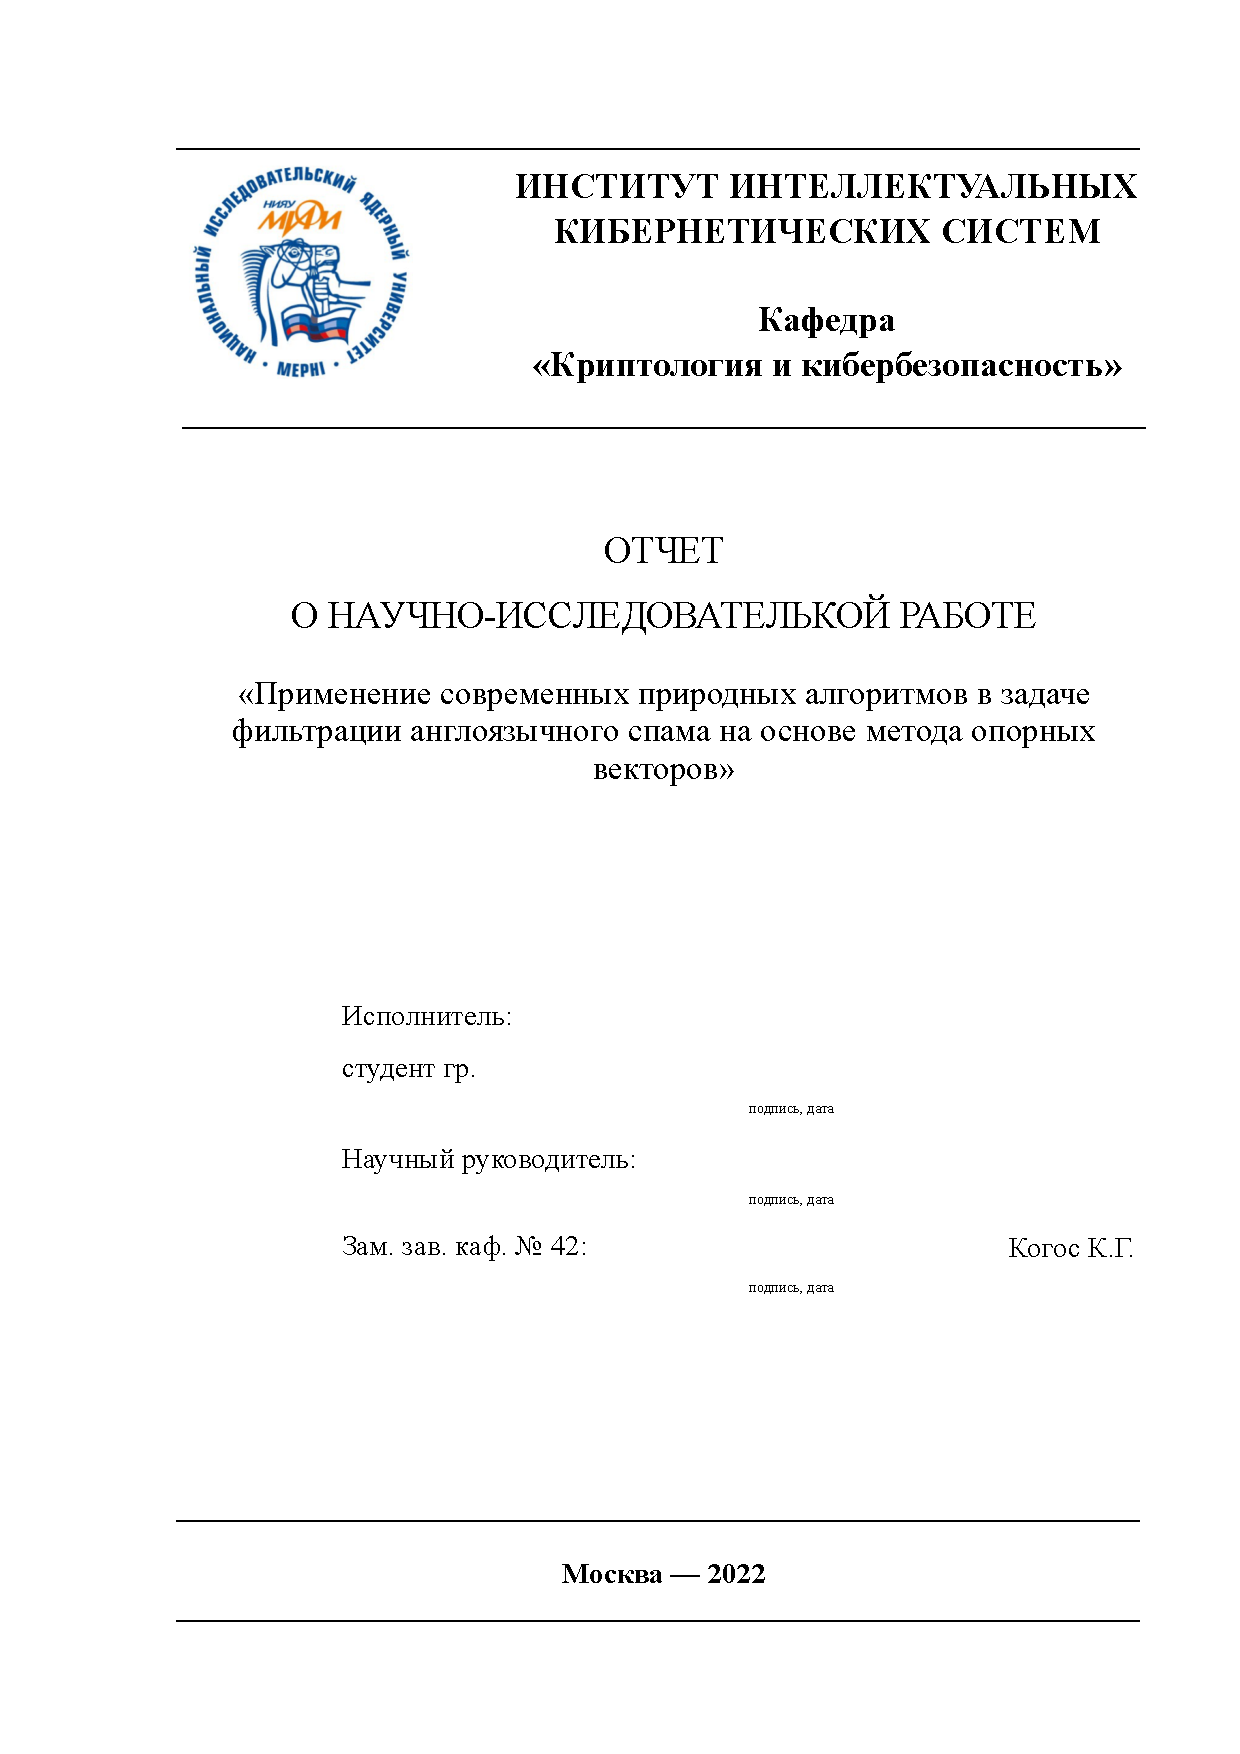
\includepdf[pages={1}]{\pwd/title.pdf}

\setcounter{page}{2}

% реферат
\clearpages
\chapter*{Реферат}
\thispagestyle{plain}
Пояснительная записка содержит 68 страниц, 11 рисунков, 2 таблицы, 2 приложения и 27 источников.

Ключевые слова: СПАМ, МАШИННОЕ ОБУЧЕНИЕ, МЕТОД ОПОРНЫХ ВЕКТОРОВ, ОПТИМИЗАЦИЯ, 
ПРИРОДНЫЙ АЛГОРИТМ, ГИПЕРПАРАМЕТР, ACCURACY, PRECISION, RECALL, F1-SCORE.

Целью работы является выявление наиболее эффективного нового природного алгоритма 
для классификации англоязычного спама на основе метода опорных векторов. 

Объект исследования — классификаторы спама на основе машинного обучения. 

Предмет исследования — оптимизация гиперпараметров алгоритмов машинного обучения.

Методы исследования — анализ существующих подходов к оптимизации гиперпараметров, 
создание системы подбора гиперпараметров с применением природных алгоритмов.

Результатом данной работы является сравнительная оценка эффективности современных 
природных алгоритмов при решении задачи распознавания англоязычного спама.

Качественный подбор параметров алгоритма машинного обучения является актуальной задачей, 
поскольку они во многом определяют точность работы получившегося спам-классификатора.

% содержание
\clearpage
\tableofcontents{}

% Определения, обозначения, сокращения
\clearpage
\chapter*{Определения, обозначения и сокращения}\addcontentsline{toc}{chapter}{Определения, обозначения, сокращения}

В настоящем отчете применяются следующие термины с соответствующими определениями, 
обозначениями и сокращениями:

\begingroup
\setlength{\baselineskip}{1.5em}
\renewcommand{\arraystretch}{1.5}
\begin{table}[ht]
    % \centering
    \begin{tabular}{ p{0.1\textwidth} p{0.03\textwidth} p{0.8\textwidth} } 
        Спам & — & нежелательные сообщения, массово рассылаемые по электронной почте \\
        МО & — & машинное обучение \\
        MTA & — & агент передачи сообщений, программное обеспечение, которое передает сообщения электронной почты с одного компьютера на другой с помощью SMTP (Message Transfer Agent) \\
        SI & — & роевой интеллект, коллективное поведение 
        децентрализованных, самоорганизованных систем, естественных или 
        искусственных (Swarm Intelligence) \\
        AO & — & Оптимизатор орла (Aquila optimizer) \\
        HGS & — & Поиск голодных игр (Hunger Games Search) \\
        SSA & — & Алгоритм поиска воробьев (Sparrow Search Algorithm) \\
        MRFO & — & Алгоритм оптимизации кормодобывания скатов манта (Manta Ray Foraging Optimization) \\
        SVM & — & Метод опорных векторов (Support vector machine) \\
        SGD & — & Стохастический градиентный спуск (Stochastic gradient descent) \\
    \end{tabular} 
\end{table}
\endgroup

% введение
\clearpage
\chapter*{Введение}\addcontentsline{toc}{chapter}{Введение}

В разделе \ref{Chapter:Analysis} .

В разделе \ref{Chapter:Theory} .

В разделе \ref{Chapter:Ingeneering} .

В разделе \ref{Chapter:Implementation} . 


% обзор на фильтрацию
\clearpage
\section{Классификация методов фильтрации спама в электронной почте}\label{Section:Filtering}

Одна из причин, по которой спам трудно фильтровать, заключается в
его динамическом характере. Характеристики спама, такие как темы,
повторяющиеся термины и т. д., в электронной почте быстро меняются
со временем, поскольку появляются новые способы обхода спам-фильтров.
Эти способы включают: обфускацию слов, спам в виде изображений,
рассылку спама по электронной почте с взломанных компьютеров и другие.
Понимание природы и эволюции спама может помочь в разработке мер
противодействия. Нет универсального метода защиты от спама, однако
наилучший подход должен обладать механизмом для определения эволюции
характеристик спама. Среди всех традиционных подходов огромного успеха
в борьбе со спамом удалось достичь благодаря фильтрации на основе
содержимого, в частности, системам на основе машинного обучения.
Они обучаются и адаптируются к новым угрозам, реагируя на меры
противодействия спамеров.

Согласно работе \cite{filters}, классификация методов фильтрации спама включает в себя подходы
на основе репутации, на основе текстового содержимого и на основе машинного обучения.

\subsection{На основе репутации (Reputation-based)}

Фильтрация на основе репутации включает в себя анализ источника сообщения, анализ социальных сетей,
анализ трафика и анализ протокола.

\subsubsection{Анализ источника сообщения}

Анализ источника сообщения включает в себя:

\begin{itemize}
    \item[—] Blacklisting — создание и поддержание на уровне пользователя
        или сервера списка адресов электронной почты или IP-адресов сервера,
        с которого, как установлено, исходит спам. Сообщение автоматически
        блокируется на этапе подключения SMTP;
    \item[—] Whitelisting — в противоположность черному списку, список
        предварительно утвержденных или доверенных контактов, доменов или
        IP-адресов, которые могут общаться с пользователем почты.
\end{itemize}


\subsubsection{Анализ социальных сетей}
Социальные сети очень полезны для определения
надежности отправителей, поэтому в подходах к фильтрации спама стали использоваться
взаимодействия в социальных сетях. Например, можно анализировать поля заголовка
электронной почты, чтобы построить граф социальной сети пользователя, а затем классифицировали
сообщения электронной почты на основе «коэффициента кластеризации» подкомпонента графа;

\subsubsection{Анализ трафика}

Анализ трафика включает в себя следующие подходы:

\begin{itemize}
    \item[—] Анализ объема писем — такой фильтр использует алгоритм, который проверяет,
        сколько электронной почты получено от определенного хоста во время последних
        подключений. Если полученное количество писем превышает определенный порог,
        оно классифицируется как спам. Этот фильтр смог правильно классифицировать
        все допустимые электронные письма для достаточно высокого порога. Недостатком
        этого фильтра является то, что при его использовании много ложных срабатываний \cite{IFIP};
    \item[—] SMTP Flow — анализ пути SMTP работает путем изучения «спамовости» или легитимности
        IP-адресов путем изучения истории электронной почты, доставленной через этот IP-адрес.
        Анализ SMTP-трафика при использовании в сочетании с традиционными фильтрами
        действительно повышает точность фильтров.
\end{itemize}

\subsubsection{Анализ протокола}

Анализ протокола включает в себя:

\begin{itemize}
    \item[—] C/R (challenge-response) systems — это спам-фильтр, который автоматически отправляет
        ответ с запросом (предполагаемому) отправителю входящего электронного письма. В этом
        ответе предполагаемого отправителя просят выполнить некоторые действия, чтобы гарантировать
        доставку исходного сообщения, которое в противном случае не было бы доставлено. Действие, которое
        нужно выполнить, может варьироваться от простого вопроса до \emph{CAPTCHA} («Полностью автоматизированный
        общедоступный тест Тьюринга, позволяющий отличить компьютеры от людей»). Отправитель обязан правильно
        ответить в своем ответе; иначе его сообщение будет удалено или помещено в папку для спама. Хотя этот
        метод эффективен для перехвата спама из автоматических систем или бот-сетей, он приводит к нежелательной
        задержке в процессе доставки.
        Системы C/R — противоречивые решения, и их часто критикуют из-за неудобств, связанных с накладными расходами
        на связь. Кроме того, могут быть заблокированы легальные электронные письма из автоматических списков
        рассылки, так как они не справятся с задачей;
    \item[—] SMTP Flow — когда SMTP-клиент подключается в первый раз, сер-\\вер-получатель может проверить,
        заблокирован ли IP-адрес отправителя или его адрес электронной почты или предварительно одобрен.
        Может быть и так, что их нет ни в черном, ни в белом списке. В этом случае сообщение временно отклоняется,
        и получатель отвечает сообщением о временной ошибке SMTP. Затем MTA-получатель записывает идентичность недавних 
        попыток, и его базы данных обновляются информацией о новых клиентах; в соответствии с требованиями SMTP RFC, 
        клиент пытается повторить попытку позже. Следующая попытка может быть принята за законных отправителей. 
        Хотя этот прием кажется очень эффективным, уклониться от него тоже очень просто. Для повторной попытки спамеры 
        могут использовать зомби.
\end{itemize}

\subsection{На основе текстового содержимого}
Фильтрация на основе текстового содержимого включает в себя эвристические и fingerprint-based фильтры.

\subsubsection{Эвристические фильтры}
Первоначально спам-фильтры следовали подходу «инженерии знаний» и основывались
на закодированных правилах или эвристиках. Эвристический фильтр на основе содержимого анализирует содержимое сообщения
и классифицирует его как спам или обычное письмо, основываясь на появлении в нем «спамных» слов, таких
как «виагра» или «лотерея». Они были разработаны на основе знания закономерностей, наблюдаемых в
сообщениях.

Недостатком эвристических фильтров является то, что разработка эффективного набора правил — трудоемкое
дело, более того, правила необходимо постоянно обновлять, чтобы идти в ногу с новейшими тенденциями в
области спама. Спамеры начали использовать «обфускацию» контента, маскируя определенные термины,
которые очень распространены в спам-сообщениях. Более того, написание правил, основанных на регулярных
выражениях, затруднено и подвержено ошибкам. Несмотря на эти ограничения, решение для фильтрации на
основе правил пользовалось успехом с 2004 года до конца прошлого десятилетия.

\subsubsection{Fingerprint-based фильтры}
К данной категории относятся следующие подходы:

\begin{itemize}
    \item[—] Honeypots (приманки) — это сервер-ловушка или система, настроенная исключительно для сбора спама или
        информации о злоумышленниках. Он также используется для идентификации сборщиков адресов электронной
        почты с помощью специально созданных адресов электронной почты и для обнаружения ретрансляторов
        электронной почты. Большинство ловушек-приманок — это бездействующие учетные записи электронной почты,
        логика которых заключается в том, что, если мертвый почтовый ящик не может согласиться на получение
        электронной почты, любой, кто отправляет это письмо, должен быть спамером;
    \item[—] Подход на основе сотрудничества — спамеры обычно рассылают спам огромному количеству получателей. Вполне вероятно, что такой же спам
        был получен кем-то другим. Совместная фильтрация спама — это распределенный подход к фильтрации спама,
        при котором все сообщество работает вместе, имея общие знания о спаме. Подход на основе сотрудничества
        не учитывает содержание электронных писем; скорее, для этого требуется накопление любой идентифицирующей
        информации, касающейся спам-сообщений, например — тема, отправитель, результат вычисления математической
        функции над телом электронного письма и т. д. Спам-сообщения имеют цифровые следы, которые делятся с
        сообществом ранние приемники. Затем пользователи сообщества используют эти отпечатки пальцев спама для
        идентификации электронных писем со спамом. Однако такие схемы страдают от проблем с
        масштабируемостью и некоторых лежащих в основе неявных предположений;
    \item[—] Подход на основе сигнатур — множество антивирусных продуктов работают на основе сигнатур. Хеши ранее
        идентифицированных спам-сообще-\\ний хранятся в базе данных на уровне MTA. Все входящие сообщения
        электронной почты проверяются по этим хешам. Поскольку сигнатуры точно соответствуют шаблонам,
        эта схема может обнаруживать известный спам с очень высокой степенью уверенности.
        Однако серьезным недостатком является то, что неизвестный или вновь созданный спам сможет
        пройти через этот фильтр, не будучи обнаруженным. Базы сигнатур необходимо постоянно обновлять.
        Кроме того, спамеры могут вводить случайную строку в спам-сообщения для генерации различных хешей.
\end{itemize}

\subsection{Фильтрация на основе машинного обучения}
Алгоритмы машинного обучения достигли наибольшего успеха среди
всех предыдущих методов. Некоторые из них будут рассмотрены в следующем разделе.


% обзор на алгоритмы МО
\clearpage
\setcounter{chapter}{1}
\setcounter{section}{0}
\chapter*{Обзор алгоритмов фильтрации спама на основе машинного обучения}\label{Chapter:ML}
Алгоритмы машинного обучения достигли наибольшего успеха среди всех 
перечисленных ранее методов, использованных в задаче фильтрации спама 
\cite{filters}. Сегодня самые успешные спам-фильтры используют машинное обучение.
\section{Фильтрация спама как задача машинного обучения}
Автоматическая классификация электронной почты использует статистические подходы 
или методы машинного обучения и направлена ​​на построение модели или классификатора 
специально для задачи фильтрации спама из потока почты пользователей.

С точки зрения машинного обучения, фильтрация спама — это задача классификации, 
в которой легитимные сообщения электронной почты рассматриваются как отрицательные 
(-) экземпляры, а спам - как положительные (+). 
Для построения модели или классификатора требуется набор предварительно классифицированных 
документов (обучающий набор). Процесс построения модели называется обучением. 
В задаче бинарной классификации алгоритм МО сначала тренируется на объектах из 
обучающей выборки, для которых заранее известны метки классов. Затем для каждого 
объекта из тестового набора данных обученный алгоритм предсказывает метку класса. 

Успех алгоритмов машинного обучения в области фильтрации спама отчасти связан с тем, что 
обучить и построить классификатор для сообщений электронной почты, получаемых отдельными 
пользователями, легче,  чем создавать и настраивать набор правил фильтрации. Кроме того, 
спам-фильтры на основе машинного обучения переобучаются при использовании и сводят к 
минимуму ручные усилия.

% виды МО (с учителем наблюдателем и тд)

\section{Некоторые из популярных методов МО в фильтрации спама}
Для проведения эксперимента будет использована библиотека языка Python Scikit-Learn.
В дальнейшем программные скрипты будут реализованы с использованием методов 
оптимизации и сравнены с параметрами по умолчанию.

\subsection{Наивный Байесовский классификатор (NBC)}
Классификатор был впервые разработан в 1990-х годах, и наиболее известен 
своим применением как один из первых методов фильтрации спама. \cite{Bayes}
При Байесовском подходе максимизируется апостериорная вероятность класса.

В естественном языке вероятность появления определенного слова в письме 
сильно зависит от контекста. Байесовский классификатор представляет письмо 
как набор слов, вероятности появления которых условно не зависят друг от друга. 
Такой подход также называется моделью "Мешок слов". 
Исходя из предположения о независимости, условная вероятность принадлежности 
письма к категории спама аппроксимируется произведением условных 
вероятностей всех входящих в него слов.

Теорема Байеса применительно к задаче классификации спама, имеет вид:
\begin{equation}\label{eq1}
    P(Class | WORD) = \frac{P(WORD | Class) \times P(Class)}{P(WORD)}
\end{equation}
Где:
\begin{itemize}
    \item[\bullet] ${WORD}$ -- это $({word_1}, {word_2}, \dots {word_n})$;
    \item[\bullet] ${«Class»}$ -- либо ${«Spam»}$, либо ${«Ham»}$;
    \item[\bullet] ${P(Class | WORD)}$ -- условная вероятность того, что письмо принадлежит классу ${Class}$;
    \item[\bullet] ${P(WORD | Class)}$ -- вероятность обнаружить письмо среди всех писем класса ${Class}$;
    \item[\bullet] ${P(Class)}$ -- полная вероятность встретить письмо класса ${Class}$ в корпусе писем;
    \item[\bullet] ${P(WORD)}$ -- безусловная вероятность письма в корпусе писем;
\end{itemize}

Предположение о независимости:
\begin{equation}\label{eq2}
    P(WORD | Spam) \approx P(word_1 | Spam) \dots P(word_n | Spam) = \prod_{i=1}^n P(word_i | Spam)
\end{equation}

Если ${Class = Spam}$, уравнение \ref{eq1} примет вид:
\begin{equation}\label{eq3}
    P(Spam | WORD) = \frac {\prod_{i=1}^n P(word_i | Spam) \times P(Spam)} {P(word_1, \dots ,word_n)}
\end{equation}

Существует три типа наивных байесовских классификаторов: мультиномиальные, 
гауссовские и Бернулли. Для идентификации спама в электронной почте 
был выбран полиномиальный наивный байесовский алгоритм, поскольку он 
связан с текстом и превосходит по своим характеристикам гауссовский 
алгоритм и алгоритм Бернулли \cite{IEEE}.

Несмотря на свои явно чрезмерно упрощенные предположения, 
наивные байесовские классификаторы довольно хорошо работают 
во многих реальных ситуациях, в том сичле, при фильтрации 
спама. Им также требуется небольшой объем обучающих 
данных для оценки необходимых параметров. \cite{scikit}

\subsection{Мультиномиальный наивный Байесовский классификатор (MNB)}
В задачах классификации текста данные обычно представлены как счетчики векторов слов. 
Распределение параметризуется векторами $\theta_y = (\theta_{y1},\ldots,\theta_{yn})$ 
для каждого класса ${y}$, где ${n}$ - количество функций (в 
классификации текста - размер словаря) и $\theta_{yi}$ это вероятность 
$P(x_i \mid y)$ признака ${i}$ из выборки, принадлежащей к классу ${y}$.
Параметры $\theta_y$ оценивается сглаженной версией максимального правдоподобия, 
то есть подсчетом относительной частоты:

\begin{equation}\label{eq4}
    \hat{\theta}_{yi} = \frac{ N_{yi} + \alpha}{N_y + \alpha n}
\end{equation}

Где:
\begin{itemize}
    \item[\bullet] $N_{yi} = \sum_{x \in T} x_i$ -- это количество раз, 
    которое появляется признак ${i}$ в образце класса ${y}$
    \item[\bullet] $N_{y} = \sum_{i=1}^{n} N_{yi}$ -- общее количество всех признаков для класса ${y}$
\end{itemize}

Сглаживающий параметр $\alpha \ge 0$ учитывает особенности, отсутствующие 
в обучающих выборках, и предотвращает нулевые вероятности в дальнейших 
вычислениях. Параметр $\alpha = 1$ называется сглаживанием Лапласа, а $\alpha < 1$ 
называется сглаживанием Лидстоуна. \cite{scikit}

\subsection{Машины опорных векторов (SVM)}
В отличие от наивного Байеса, SVM -- не вероятностный алгоритм.

Гиперплоскость -- пространство размерностью на единицу меньше размерности исходного пространства.
Основная цель машины опорных векторов в задаче бинарной классификации —- найти 
уравнение разделяющей гиперплоскости $w_1x_1+w_2x_2+…+w_nx_n+w_0=0$ 
в пространстве $R^n$, которая бы разделила два класса неким оптимальным образом. 

Возможные значения меток классов $Y = \{-1, +1\}$. Объект —- вектор в пространстве $R^n$ c 
N признаками $x = (x_1, x_2, \dots, x_n)$. Алгоритм при обучении должен построить функцию 
$F(x)=y$, аргументом $x$ которой является объект из пространства $R^n$, а результатом -- метка класса $y$.

Любая гиперплоскость может быть задана в виде $\langle w, x \rangle + b$.
Метод опорных векторов строит классифицирующую функцию

% \begin{equation}\label{eq5}
    \[F(x) = sign(\langle w, x \rangle + b)\]
% \end{equation}

Где: 
\begin{itemize}
    \item[\bullet] $\langle , \rangle$ — скалярное произведение;
    \item[\bullet] $w$ -— нормальный вектор к разделяющей гиперплоскости;
    \item[\bullet] $b$ — вспомогательный параметр;
\end{itemize}

Объекты, для которых $F(x) = 1$, оказываются по одну сторону гиперплоскости, 
то есть попадают в один класс, а объекты с $F(x) = -1$ —- по другую, соответственно, 
попадают в другой класс.

$w$ и $b$ выбираются таким образом, чтобы максимизировать расстояние до каждого класса. 
Другими словами, алгоритм максимизирует отступ (англ. \emph{margin}) между гиперплоскостью 
и объектами классов, расположенными к ней ближе всего. Такие объекты называются опорными векторами \emph{(support vectors)}.
Расстояние до каждого класса равно $\frac {1}{\Arrowvert w \Arrowvert}$. Проблема нахождения максимума 
$\frac {1}{\Arrowvert w \Arrowvert}$ эквивалентна проблеме нахождения минимума ${\Arrowvert w \Arrowvert}^2$. 
Задача оптимизации:
\begin{equation}\label{eq6}
    \left\{ \begin{array}{ll} arg \: \underset{w,b}{\min} {\Arrowvert w \Arrowvert}^2 & \textrm{}\\ y_i(\langle w,x_i \rangle + b) \geqslant 1, \: i = 1, \dots, m \end{array} \right.
\end{equation}
решается с помощью множителей Лагранжа.

В случае линейной неразделимости, когда данные нельзя разделить гиперплоскостью, поступают 
все элементы обучающей выборки вкладываются в пространство $X$ более высокой размерности с 
помощью специального отображения $\varphi : R^n \rightarrow X$, которое выбирается таким образом, 
чтобы выборка была линейно разделима в $X$.

Классифицирующая функция $F$ принимает вид $F(x)=sign(\langle w, \varphi (x) \rangle + b)$. 
Ядро \emph{(kernel function)} классификатора: $k(x, x') = \langle \varphi (x), \varphi (x') \rangle $.
Ядром может служить любая положительно определенная симметричная функция двух переменных. 
В разных алгоритмах SVM используются разные типы функций ядра. Например, линейная, нелинейная, 
полиномиальная, радиальная базисная функция (RBF) и сигмоид. \cite{SVM}

Машины опорных векторов (SVM) считаются одним из лучших алгоритмов обучения 
с учителем. Они обеспечивают превосходную производительность обобщения, требуют 
меньше примеров для обучения и могут обрабатывать многомерные данные. \cite{scikit}

Гиперплоскость можно описать уравнением:
\begin{equation}\label{eq5}
    H = VX + c (5)
\end{equation}
где $c$ -- постоянная, а $V$ -- вектор.

Алгоритм использует скорость обучения для итерации по образец данных для 
оптимизации линейного алгоритма, и он обозначается следующим уравнением-6 
для скорости обучения по умолчанию как «Оптимальный»:

\section{Метрики машинного обучения}


\section{Выбор алгоритма МО для эксперимента}
Наивный байесовский классификатор (NB) - это простой, но эффективный классификатор, 
который использовался во многих приложениях обработки информации, включая обработку 
естественного языка, поиск информации и т. д. Данныцй метод особенно подходит для решения задач 
с большим объемом входных данных.



% обзор на природные алгоритмы
\clearpage
\section{Алгоритмы оптимизации}\label{Section:Bio}

В последние годы в литературе описано большое количество алгоритмов,
основанных на природе и биологии. Это семейство алгоритмов симулирует
различные биологические процессы, наблюдаемые в природе, чтобы решать
сложные задачи оптимизации \cite{Yang2009}. Каждый естественный процесс
можно считать адаптируемым и имитируемым для создания нового
метаэвристического подхода, но с различными возможностями достижения
глобальных оптимальных решений для задач оптимизации \cite{BioInspiredTaxonomy}.

\subsection{Задача оптимизации}

Без преувеличения можно сказать, что в оптимизация используется повсюду: от
инженерного проектирования до бизнес-планирования и маршрутизации
Интернета до планирования праздников. Почти во всех этих действиях мы
пытаемся достичь определенных целей или оптимизировать что-то, например
прибыль, качество и время. Поскольку в реальных приложениях ресурсы,
время и деньги всегда ограничены, мы должны найти решения для оптимального
использования этих ценных ресурсов при различных ограничениях.
Математическая оптимизация или программирование — это изучение таких
проблем планирования и проектирования с использованием математических
инструментов. В настоящее время компьютерное моделирование становится
незаменимым инструментом для решения таких задач оптимизации с помощью
различных эффективных алгоритмов поиска.

С математической точки зрения, большинство задач оптимизации можно описать
в общем виде:

\begin{equation}\label{eq7}
    \underset{X \in R^n}{minimize} \: f_i(X), (i=1,2,\dots,M),
\end{equation}

\begin{equation}\label{eq8}
    subject\: to \: h_j(X) = 0, (j=1,2,\dots,J),
\end{equation}

\begin{equation}\label{eq9}
    g_k(X) \leq 0, (k=1,2,\dots,K)
\end{equation}

Где $f_i(X), h_j(X), g_k(X)$ — функции порождающего вектора

\begin{equation}\label{eq10}
    X = (x1,x2,\dots,x_n)^T
\end{equation}

Здесь компоненты $x_i$ переменной $x$ называются переменными решения.
Функции $f_i(x)$, где $i = 1, 2, \dots, M$, называются \emph{целевыми функциями}
или функциями стоимости. Пространство, охватываемое переменные решения,
называется \emph{пространством поиска} $R^n$, а пространство, образованное значениями
целевых функций, называются \emph{пространством решений} или пространством ответов.
Равенство \eqref{eq8} с $h_j$ и неравенство \eqref{eq9} с $g_k$ называются \emph{ограничениями}.

Проблемы оптимизации обычно описывают в терминах локальной или глобальной
оптимизации:

\begin{itemize}
    \item[—]
        \emph{Локальная оптимизация}, при которой алгоритм ищет точку, которая является
        только локально оптимальной, что означает, что она минимизирует целевую
        функцию среди возможных точек, которые находятся рядом с ней. Методы локальной оптимизации широко используются в приложениях, где есть смысл
        найти хорошую, если не самую лучшую точку \cite{Boyd2004};

    \item[—]
        \emph{Глобальная оптимизация}, при которой алгоритм ищет глобальный оптимум,
        используя механизмы для поиска в более крупных частях пространства поиска.
        Глобальная оптимизация используется для задач с небольшим количеством
        переменных, где время вычислений не критично, а ценность поиска истинного
        глобального решения очень высока \cite{Boyd2004}.
\end{itemize}

\subsection{Классификация алгоритмов оптимизации}

Также алгоритмы оптимизации можно разделить на \emph{детерминированные} и
\emph{стохастические}. В отличие от детерминированных моделей,
которые дают одинаковые точные результаты для определенного набора
входных данных, стохастические модели представляют данные и
предсказывают результаты, учитывающие определенные уровни
непредсказуемости или случайности.

Стохастические алгоритмы бывают \emph{эвристические} и \emph{метаэвристические}.
Можно сказать, что эвристика использует зависящую от проблемы информацию
для поиска «достаточно хорошего» решения конкретной проблемы, в
то время как метаэвристика представляет собой общие алгоритмические
идеи, которые можно применять к широкому кругу проблем.

Стоит отметить, что в литературе не существует согласованных определений
эвристики и метаэвристики. Некоторые используют термины «эвристика» и
«метаэвристика» как синонимы. Однако в последнее время все стохастические
алгоритмы с рандомизацией и локальным поиском называются
метаэвристическими \cite{Yang2009}.

\subsection{Оптимизация гиперпараметров в машинном обучении}\label{optimization}

Гиперпараметр модели — это параметр, который является внешним по
отношению к модели и значение которого невозможно оценить по данным.
Мы не можем знать наилучшее значение гиперпараметра модели для той или иной проблемы.
Часто гиперпараметры можно установить с помощью эвристики.

К основным подходам к оптимизации гиперпараметров относятся:

\begin{itemize}
    \item[—] \emph{Поиск по сетке} представляет собой простой перебор
        по заданному вручную подмножеству гиперпараметрического пространства
        алгоритма обучения;
    \item[—] \emph{Случайный поиск} заменяет перебор всех комбинаций их случайным выбором;
    \item[—] \emph{Градиентный спуск} — для конкретных алгоритмов МО (например, метод опорных векторов)
        можно вычислить градиент относительно гиперпараметров, а затем
        оптимизировать гиперпараметры с помощью градиентного спуска;
    \item[—] Идея \emph{байесовской оптимизации} состоит в построении
        вероятностной модели целевой функции и использовании ее для выбора
        наиболее подходящих гиперпараметров;
    \item[—] \emph{Эвристический подход} подразумевает применение различных эвристическикх и
        метаэвристических алгоритмов оптимизации.
\end{itemize}

\subsection{Природные алгоритмы оптимизации}

Как уже было сказано, оптимизация гиперпараметров — это поиск набора переменных, который позволит
алгоритму достичь более качественных результатов. Гиперпараметры обычно оказывают
значительное влияние на успех алгоритмов машинного обучения.
При оптимизации гиперпараметров возможно использование более сложных алгоритмов, 
чем поиск по сетке или случайный поиск. В частности, природных алгоритмов.

Классифицировать природные алгоритмы можно по разным признакам, однако наиболее
часто этим признаком служит биологический источник вдохновения \cite{BioInspiredTaxonomy}.

\subsubsection{Эволюционные алгоритмы}

В эту категорию входят алгоритмы, основанные на популяциях, а также
на принципах естественной эволюции. К ним относятся как
классические алгоритмы эволюционных вычислений, такие как генетический
алгоритм (GA), стратегии эволюции (ES) и дифференциальная эволюция (DE),
таки менее известные алгоритмы, основанные на воспроизведении
различных биологических организмов, таких как пчелиные матки и сорняки.

\subsubsection{Алгоритмы на основе роевого интеллекта}

Роевой интеллект (SI) — это уже устоявшийся термин. Его можно определить
как коллективное поведение децентрализованных, самоорганизованных систем в
естественной или искусственной среде. Выражение было предложено в контексте
роботизированных систем, но с годами обобщено, чтобы обозначить возникновение
коллективного разума из группы простых агентов, управляемых простыми поведенческими
правилами. Таким образом, биологические метаэвристики, относящиеся к роевому
интеллекту, основаны на коллективном поведении сообществ животных, таких как
колонии насекомых или стаи птиц, в которых коллективный разум позволяет решать
задачи оптимизации.

Разделение на подкатегории по среде может быть следующим:

\begin{itemize}
    \item[—] Летающие животные

        Эта категория включает в себя метаэвристику, основанную на
        концепции роевого интеллекта, в которой траектория агентов
        определяется полетом, как у птиц, летучих мышей или других
        летающих животных. Самыми известными алгоритмами в этой
        подкатегории являются метод роя частиц (PSO) [2] и алгоритм пчелиной
        колонии (ABC);

    \item[—] Наземные животные

        Метаэвристика в этой категории основана на поисках пищи или
        передвижениях наземных животных. Наиболее известным подходом в
        этой категории является муравьиный алгоритм (ACO),
        который воспроизводит механизм, используемый муравьями для
        определения местоположения источников пищи и
        информирования об их существовании своим собратьям в колонии.
        В эту категорию также входят другие популярные алгоритмы, такие
        как алгоритм стаи серых волков (GWO), алгоритм льва (LOA),
        которые имитируют методы охоты, используемые этими животными;

    \item[—] Водные животные

        Этот тип метаэвристических алгоритмов основан на поведении водных животных.
        Сюда относятся такие популярные алгоритмы, такие как
        стадо криля (KH), алгоритм китов (WOA), а также алгоритмы,
        основанные на эхолокации, используемой дельфинами для обнаружения рыб,
        такие как оптимизация партнеров дельфинов (DPO) и эхолокация дельфинов (DEO);

    \item[—] Микроорганизмы

        Метаэвристика, основанная на микроорганизмах, связана с поиском пищи
        бактериями. Колония бактерий совершает движение в поисках пищи. Другие
        типы метаэвристик, которые могут быть частью этой категории,
        связаны с вирусами, которые обычно воспроизводят процесс заражения клетки
        вирусом. Наиболее известным алгоритмом этой категории является алгоритм
        оптимизации сбора бактерий (BFOA).

\end{itemize}


При разделении на подкатегории по вдохновляющему поведению каждый
алгоритм классифицируется как принадлежащий к одному из следующих
поведенческих паттернов:

\begin{itemize}
    \item[—] Движение

        Алгоритм относится к подкатегории
        движения, если биологическое вдохновение в основном состоит в
        том, как животное перемещается в окружающей среде;

    \item[—] Собирательство

        В алгоритмах на основе собирательства поведение животного определяет
        механизм, используемый для получения пищи.

\end{itemize}


\subsubsection{Алгоритмы на основе физики / химии}

Алгоритмы этой категории характеризуются тем, что они имитируют поведение
физических или химических явлений, таких как гравитационные силы,
электромагнетизм, электрические заряды и движение воды, а также химические
реакции и движение частиц газа. В этой категории мы можем найти
некоторые хорошо известные алгоритмы, разработанные в прошлом веке,
такие как алгоритм имитации отжига (SA) или алгоритм гравитационного поиска (GSA).
Другие алгоритмы, такие как гармонический поиск (HS), относятся к процессу сочинения
музыки, человеческому изобретению, которое имеет больше общего с другими
физическими алгоритмами в том, что касается использования звуковых волн,
чем с алгоритмами, основанными на социальном поведении человека.

\subsubsection{Алгоритмы, основанные на социальном поведении человека}

Алгоритмы, попадающие в эту категорию, вдохновлены человеческими социальными
концепциями, такими как принятие решений и идеями, связанными с конкуренцией
идеологий внутри общества, таких как алгоритм идеологии (IA) или политическими
концепциями, такими как алгоритм империалистической колонии (ICA). В эту
категорию также входят алгоритмы, имитирующие спортивные соревнования,
такие как алгоритм футбольной лиги (SLC). Процессы мозгового штурма также заложили
вдохновляющие основы нескольких алгоритмов, таких как алгоритм оптимизации
мозгового штурма (BSO.2) и глобальный передовой алгоритм оптимизации мозгового
штурма (GBSO).

\subsubsection{Алгоритмы на основе растений}

Эта категория объединяет все алгоритмы оптимизации, поиск которых
основан на растениях. В этом случае, в отличие от методов в категории
роевого интеллекта, нет связи между агентами. Один из самых известных — это
алгоритм оптимизации леса (FOA.1), вдохновленный процессом
воспроизводства растений.

\subsubsection{Алгоритмы со смешанными источниками вдохновения}

В эту категорию входят алгоритмы, которые не подходят ни к одной из
предыдущих, то есть в ней можно обнаружить алгоритмы с различными
характеристиками, такими как оптимизация пар Инь-Ян (YYOP).
Хотя эта категория неоднородна и не демонстрирует
единообразия среди алгоритмов, которые представляет, ее включение
в классификацию служит примером очень разных источников вдохновения,
существующих в литературе. С появлением новых алгоритмов эта группа
должна дать начало новым категориям.



% оценка производительности
\clearpage
\section{Природные алгоритмы в настройке гиперпараметров}\label{Section:Performance}

Как уже было сказано, оптимизация гиперпараметров — это поиск набора переменных, который позволит
алгоритму достичь более качественных результатов. Гиперпараметры обычно оказывают
значительное влияние на успех алгоритмов машинного обучения.
Когда требуется охватить большое пространство поиска, чтобы не застрять
в локальном минимуме, и одновременно ограничить количество обучаемых
моделей до приемлемого количества, при оптимизации гиперпараметров прибегают
использованию более сложных алгоритмов, чем поиск по сетке или случайный поиск.
В частности, возможно применений природных алгоритмов.

\subsection{Оценка производительности моделей}\label{Scorer}

Для оценки производительности некоторой обученной модели можно используют определенные метрики.

\subsubsection{Матрица ошибок}

Обнаружение спама в электронных письмах можно оценить с помощью
различных показателей эффективности. Матрица ошибок используется для
визуализации работы алгоритмов и может быть определена как в Таблице \ref{table1}.

\begin{table}[!ht]
    \centering
    \caption{Матрица ошибок}
    \begin{tabular}{|p{0.3\textwidth}|p{0.3\textwidth}|p{0.3\textwidth}|}
    \hline
        — & HAM & SPAM \\ \hline
        HAM & TN & FP \\ \hline
        SPAM & FN & TP \\ \hline
    \end{tabular}
    \label{table1}
\end{table}
где:

\begin{itemize}
    \item[—] TN = TrueNegative — Письма, распознанные как письма;
    \item[—] FP = FalsePositive — Спам-письма, распознанные как письма;
    \item[—] FN = FalseNegative — Письма, распознанные как спам-письма;
    \item[—] TP = TruePositive — Спам-письма, распознанные как спам-письма.
\end{itemize}


\subsubsection{Accuracy}

Accuracy — это отношение количества правильных прогнозов к общему количеству входных
выборок \cite{scikitMetrics}:

\begin{equation}\label{eq11}
    Accuracy = {{(TN + TP)} \over{(TP + FN + FP + TN)}}
\end{equation}

\subsubsection{Recall}

Recall описывает, сколько писем было правильно отнесено к спаму из
общего количества писем, распознанных как спам $(TP + FN)$ \cite{scikitMetrics}:

\begin{equation}\label{eq12}
    Recall = {{TP} \over{(TP + FN)}}
\end{equation}

\subsubsection{Precision}

Измерение precision заключается в доли верно идентифицированного
спама из всех спам-писем $(TP + FP)$ \cite{scikitMetrics}. Определяется
уравнением:

\begin{equation}\label{eq13}
    Precision = {{TP} \over{(TP + FP)}}
\end{equation}

\subsubsection{F1-score}

Оценка $F1$ может быть интерпретирована как средневзвешенное
значение precision и recall, где оценка $F1$ достигает своего лучшего
значения при 1 и худшего значения при 0 \cite{scikitMetrics}.
Формула для оценки $F1$:

\begin{equation}\label{eq14}
    F1 = {2 \times (precision \times recall) \over{(precision + recall)}}
\end{equation}

\subsection{Переобучение}
Мы, люди, иногда склонны делать чрезмерные обобщения. К сожалению,
машины могут оказаться в такой же ситуации. В контексте МО это называется
\emph{переобучением}.

Ограничение модели с целью ее упрощения и снижения риска переобучения
называется \emph{регуляризацией} \cite{scikitBook}.

Тестирование модели на одних и тех же данных при выборе параметров является
методологической ошибкой: модель, которая будет просто повторять метки
образцов, которые она только что увидела, будет иметь идеальную оценку, но
не сможет предсказать что-либо полезное на новых данных \cite{scikitTuning}.

Чтобы решить эту проблему, еще одна часть набора данных может быть представлена
как так называемый проверочный набор \emph{(validation set)}: обучение продолжается
на обучающем наборе, после чего выполняется оценка на проверочном наборе, и
когда эксперимент кажется успешным, окончательную оценку можно провести на
тестовом наборе.


% эксперимент
\clearpage
\section{Подготовка к проведению эксперимента}

Для программной реализации системы оценки производительности 
алгоритмов оптимизации, необходимо спланировать эксперимент, 
разработать систему для проведения эксперимента, выбрать инструменты для ее реализации.

\subsection{Планирование эксперимента}

Цель эксперимента -- выявить преимущества и недостатки тех или иных видов 
оптимизации гиперпараметров и их влияния на время обучения и производительность 
модели. 

Входные данные -- набор текстов писем электронной почты, для каждого из которых 
заранее известно, является это письмо спамом или нет.

Выходные данные -- оценка нескольких обученных на входных данных классификаторов спама. 

Для удобства проведения эксперимента ограничимся алгоритмами роевого интеллекта, 
которые работают по общему принципу, а метод роя частиц уже показал хорошие 
результаты в этой области \cite{IEEE}.

План проведения эксперимента:

\begin{enumerate}
    \item Подготовить данные для эксперимента;
    \item Предварительно обработать данные. Разделить данные на тренировочный 
    и тестовый наборы;
    \item Настроить параметры алгоритма машинного обучения;
    \item Реализовать алгоритм глобальной оптимизации функции на основе того или иного природного алгоритма;
    \item Реализовать объектную функциию, подлежащую оптимизации алгоритмом роевого интеллекта.
    Эта функция должна вычислять оценку модели МО для каждой частицы с новыми параметрами, а  
    возвращать среднее арифметическое от вектора этих параметров.
    Оценочной функцией может служить как одна из \ref{Scorer}, так и 
    нестандартная весовая функция;
    \item Обучить модель с использованием полученных гиперпараметров;
    \item Протестировать модель на тестовом наборе данных;
    \item Оценить производительность модели, вычислив величины из \ref{Scorer} на 
    тестовом наборе;
    \item Повторить экспепримент, получив те же параметры с использованием 
    других подходов к оптимизации, описанных в \ref{optimization};
    \item Повторить эксперимент для другого природного алгоритма;
    \item Провести сравнительный анализ получившихся оценок с целью выявления 
    преимуществ и недостатков тех или иных видов оптимизации и их влияния на 
    время обучения и производительность модели;
    \item Объяснить полученные результаты эксперимента, сделать соответствующие выводы;
    \item Обозначить направление дальнейших исследований.
\end{enumerate}

\subsection{Архитектура системы для проведения эксперимента}

Механизм обнаружения спама должен иметь возможность работать с электронной почтой, 
включающей html-заголовки и другую лишнюю в контексте данной задачи информацию.
В связи с этим набор входных данных подлежит предварительной обработке. 

Данные также подлежат разделению на тренировочный и тестовый наборы. 

Задаются начальные параметры алгоритма, желаемое значение оценочной функции (например, $Accuracy$), 
число частиц, максимальное количество итераций. Затем на тренировочном наборе данных 
проводится обучение модели с перекрестной проверкой на различных наборах 
гиперпараметров, предоставляемых оптимизационным алгоритмом. Процесс продолжается 
до тех пор, пока не будет достигнуто желаемое значение оценки алгоритма или 
максимальное число итераций.

Затем модель, обученная на лучших параметрах, тестируется на тестовом наборе данных, 
осуществляется оценка производительности полученной модели.

Рисунок \ref{scheme} представляет процесс реализации описанной системы.

\begin{figure}[H]	
    \centering
    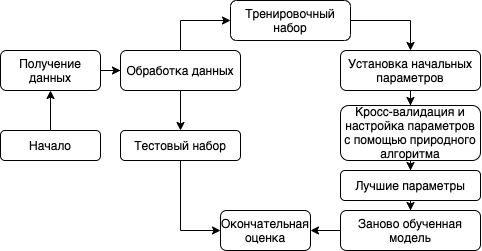
\includegraphics[width=140mm]{\pwd/prog.png}
    \caption{Схема процесса обучения модели}
    \label{scheme}
\end{figure}

\subsection{Выбор инструментов для реализации системы}

Для реализации системы выбран язык программирования Python версии 3.9 или выше, 
поскольку его использование обеспечивает наличие множества библиотек, 
предназначенных для машинного обучения. 

Реализации описанных в \ref{ML} алгоритмов машинного обучения 
можно найти в библиотеке Scikit-Learn. Scikit-Learn -- 
библиотека машинного обучения, написанная на Python, довольно популярная
среди ученых-вычислителей. Она может похвастаться простым в использовании 
интерфейсом и содержит множество инструментов для машинного обучения, в том числе 
для классификация, предварительной обработки, кластеризации и регрессии данных. 
Многие из этих алгоритмов могут быть полезны "из коробки", но чтобы получить
лучшую производительность, гиперпараметры должны быть настроены под конкретную 
проблемную область, в которой алгоритм будет использоваться. Для такой настройки 
будут использоваться алгоритмы роевого интеллекта, такие как, например, Firefly, Ant 
Colony Optimization и Bee Colony Optimization.

% алгоритмы
\clearpage
\section{Определение набора алгоритмов для проведения эксперимента}\label{BIOAlgs}

Для данной работы решено было использовать алгоритмы роевого интеллекта, опубликованные в 2020-2021 годах:

\begin{itemize}
    \item[—] AO -- Aquila Optimizer;
    \item[—] HGS -- Hunger Games Search;
    \item[—] SSA -- Sparrow Search Algorithm;
    \item[—] MRFO -- Manta Ray Foraging Optimization.
\end{itemize}

\subsection{Оптимизатор орла (Aquila optimizer)}\label{AO}

В работе \cite{AO} представлен новый метод оптимизации на основе популяций, называемый оптимизатор орла,
основанный на поведении орлов в природе во время охоты. Оптимизационные функции
данного алгоритма обусловлены четырьмя процессами: выбор пространства поиска высоким
взлетом с вертикальным наклоном, разведка в пределах расходящегося пространства поиска
контурным полетом с короткой планирующей атакой, использование в пределах сходящегося пространства
поиска низким полетом с атакой медленного спуска, а также бег и захват добычи.

\subsection{Поиск голодных игр (Hunger Games Search)}\label{HGS}

Метод оптимизации на основе популяций, называемый поиском голодных игр, основан на поведенческом выборе
животных в соответствии с чувством голода. Этот метод поиска использует простую концепцию голода как наиболее
важную гомеостатическую мотивацию и причины поведения всех живых существ. Кроме того, почти все животные используют вычислительно-логические
правила (игры). Часто такие действия являются следствиями эволюции.

Особенностью данного метода, по словам авторов, является его динамический характер, простая структура и
высокая производительность, гибкость и масштабируемость, а также тот факт, что метод был не только
проверен на хорошо известном наборе тестовых функций, но и применен к нескольким инженерным задачам \cite{HGS}.

\subsection{Алгоритм поиска воробьев (Sparrow Search Algorithm)}\label{SSA}

Алгоритм поиска воробьев представляет собой новый подход к оптимизации на основе роевого интеллекта.
Метод вдохновлен поведением воробьев в поисках пищи и в борьбе с хищниками. Авторы алгоритма
утверждают, что предлагаемый метод может обеспечить высококонкурентные результаты. Более того, результаты
двух практических инженерных задач также показывают, что алгоритм имеет высокую производительность в различных
областях поиска \cite{SSA}.

\subsection{Алгоритм оптимизации кормодобывания скатов манта (Manta Ray Foraging Optimization)}\label{MRFO}

В основе природного алгоритма оптимизации кормодобывания скатами манта (MRFO) лежит разумное поведение
скатов-мантов. Целью данного алгоритма, по утверждению авторов, является обеспечение альтернативного подхода
к оптимизации для решения реальных инженерных проблем. Производительность алгоритма была оценена
путем сравнения с другими современными оптимизаторами, с помощью функций оптимизации тестов и восьми
реальных примеров инженерного проектирования. Результаты сравнения тестовых функций показывают, что данный подход
намного превосходит своих конкурентов. Кроме того, реальные инженерные приложения демонстрируют достоинства
этого алгоритма в решении сложных проблем с точки зрения затрат на вычисления и точности решения \cite{MRFO}.



% данные
\clearpage
\section{Определение инструментов и данных}

Данный раздел описывает инструменты, используемые для программной реализации эксперимента, а
также подготовку данных.

\subsection{Оборудование и программное обеспечение}

Проект реализован на ноутбуке с 16 ГБ оперативной памяти и процессором Intel Core i7 (2,60 ГГц).
Для реализации программной системы выбран язык Python версии 3.9.7, так как данный язык 
программирования предоставляет широкий выбор библиотек для машинного обучения, в частности,
библиотеку scikit-learn. Таким образом, его использование призвано облегчить программную
реализацию алгоритмов машинного обучения и сосредоточиться непосредственно на
эксперименте.

Основные модули, использованные в работе:

\begin{itemize}
    \item[—] Mealpy — библиотека, предоставляющая реализации множества метаэвристических природных алгоритмов;
    \item[—] Nltk — библиотека для символьной и статистической обработки естественного языка для английского языка;
    \item[—] Numpy — библиотека, поддерживающая большие многомерные массивы и матрицы, а также большой набор высокоуровневых математических функций для работы с ними;
    \item[—] Pandas — библиотека для обработки и анализа данных, предлагающая, в частности, структуры данных и операции для управления таблицами и временными рядами;
    \item[—] Scikit-learn — библиотека машинного обучения, включающая в себя различные алгоритмы классификации,
        регрессии и кластеризации.
\end{itemize}

\subsection{Определение наборов данных}\label{datasets}

Для тестирования алгоритмов использовались общедоступные наборы данных, электронные
письма в которых представлены строками.
Список использованных наборов данных:

\begin{itemize}
    \item[—] Набор данных Ling-Spam (2893 писем) \cite{LingSpam};
    \item[—] Набор данных Spam-Assasin (9352 писем) \cite{SpamAssasin};
    \item[—] Набор данных Enron (33715 писем) \cite{Enron}.
\end{itemize}
% TODO здесь еще можно добавить про состав и формат датасетов
С помощью программы, приведенной в Приложении, данные были приведены к единому простому виду, содержащему поля:
содержимое письма (message) и категория (label).

Категория, в свою очередь, может принимать два значения: обычные письма (ham) и спам (spam).

Соотношение спама и обычных писем для набора данных Ling-Spam представлено на \ref{LingSpamScheme},
для Spam-assasin — на \ref{SpamAssasinScheme}, для Enron — на \ref{EnronScheme}.

\begin{figure}[H]
    \centering
    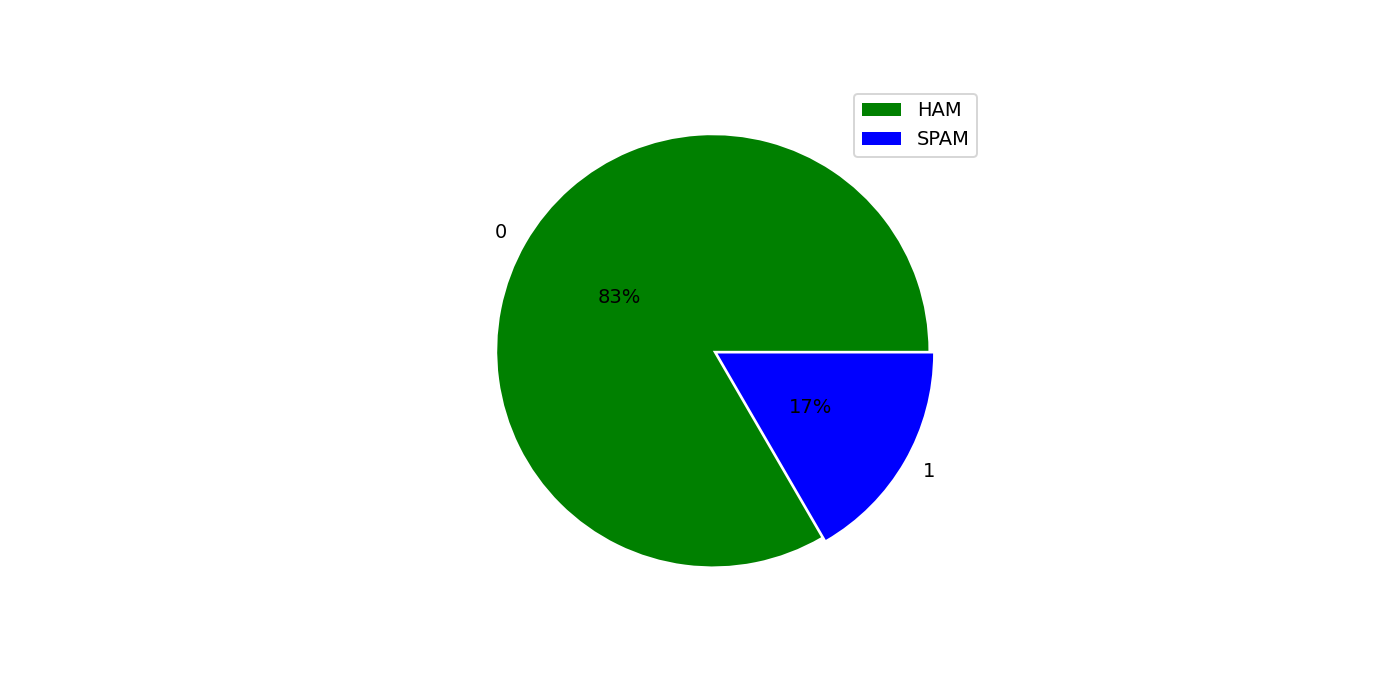
\includegraphics[width=150mm]{static/ling_spam.png}
    \caption{Соотношение спама и обычных писем для набора данных Ling-Spam}
    \label{LingSpamScheme}
\end{figure}

\begin{figure}[H]
    \centering
    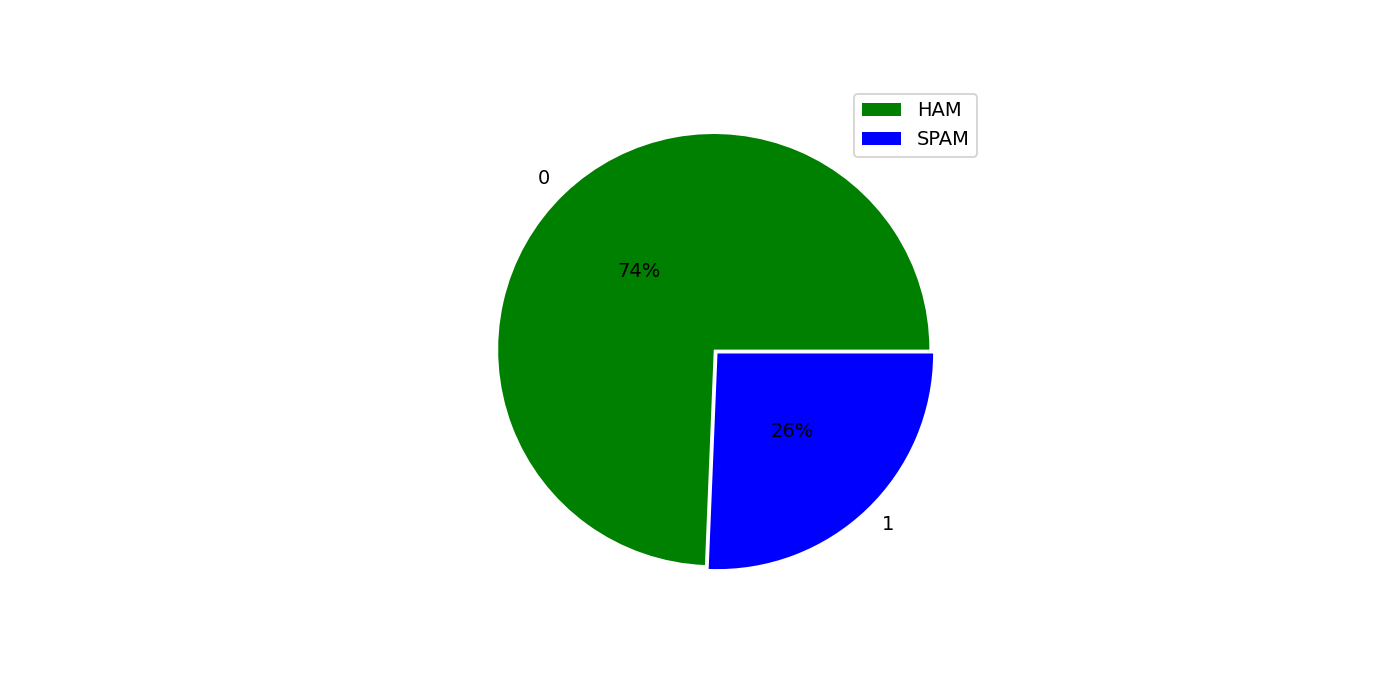
\includegraphics[width=150mm]{static/spam_assasin.png}
    \caption{Соотношение спама и обычных писем для набора данных Spam-Assasin}
    \label{SpamAssasinScheme}
\end{figure}

\begin{figure}[H]
    \centering
    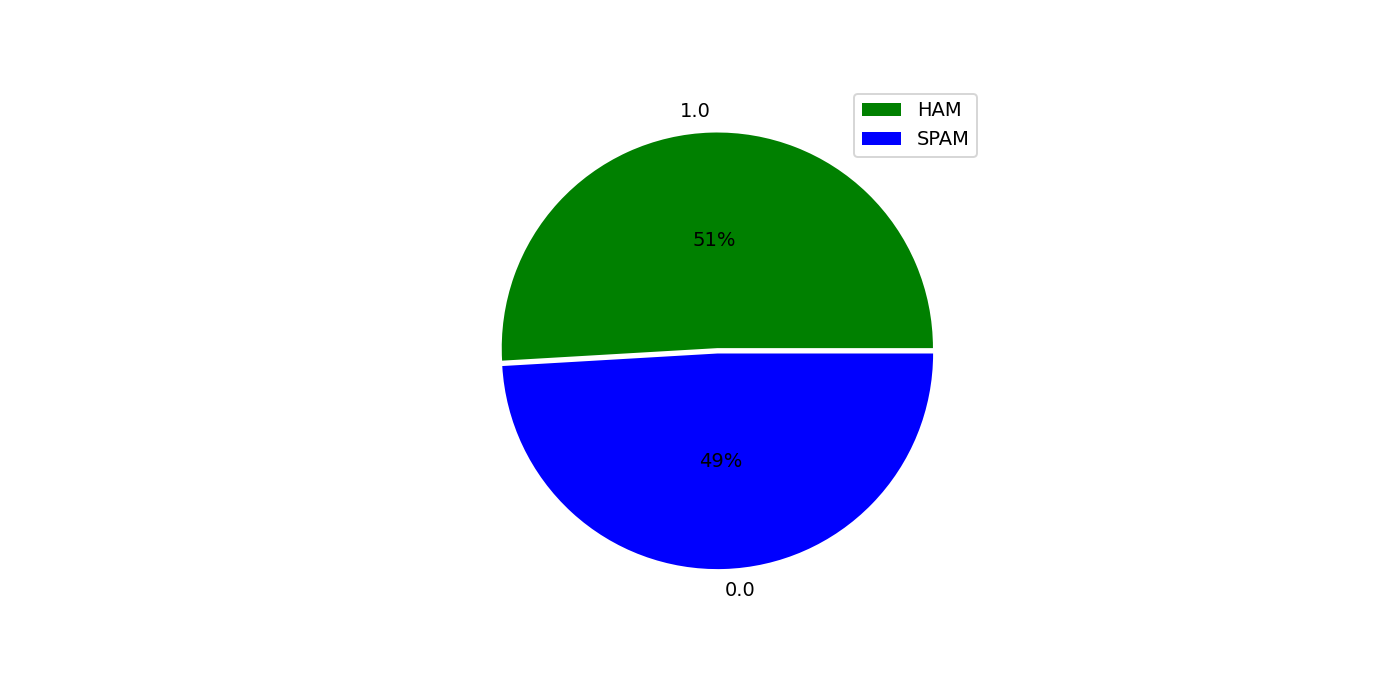
\includegraphics[width=150mm]{static/enron.png}
    \caption{Соотношение спама и обычных писем для набора данных Enron}
    \label{EnronScheme}
\end{figure}


\subsection{Предварительная обработка данных}

Текстовые данные требуют специальной подготовки, прежде чем их можно будет использовать для
моделирования.

Программную реализацию подготовки данных можно найти в \hyperref[App1]{Приложении А}.

\subsubsection{Символьная обработка}

В первую очередь необходимо очистить строки от ненужных символов. Обработка включает в себя:

\begin{itemize}
    \item[—] Замена символов переноса строки и переноса каретки пробелом;
    \item[—] Замена повторяющихся пробелов одним;
    \item[—] Удаление знаков препинания;
    \item[—] Удаление подстрок, не являющихся словами;
    \item[—] Удаление цифр;
    \item[—] Приведение всех букв к строчному виду.
\end{itemize}

\subsubsection{Токенизация}

При работе с текстовыми данными нам необходимо было представить их в виде целых чисел или чисел с плавающей точкой.
Набор текстовых документов преобразовывался в матрицу слов (токенов), из которых состоял текст. При этом нужно было также
исключить из обработки некоторые стоп-слова — различные артикли, предлоги, вводные слова. Это полезно,
поскольку такие слова не очень полезны для определения того, является ли электронное письмо спамом или нет.

Далее матрица подсчета была преобразована в нормализованное представление tf-idf. 
TF-IDF (Term Frequency - Inverse Document Frequency) — это оценка, направленная на определение важности слова
в документе, а также для учета его связи с другими документами из того же набора даннных. Tf (term frequency)
означает частоту слова, а tf-idf — это частота слова, умноженная на величину, обратную частоте,
с которой в наборе данных встречаются документы, его содержащие \cite{Manning}.

Формула, лежащая в основе статистического показателя TF-IDF:
\begin{equation}\label{eq15}
    tf-idf(w, d, D) = tf(w, d) * idf(w, D)
\end{equation}
\\
где:

\begin{itemize}
    \item[—] d — данный документ из нашего набора данных;
    \item[—] D — набор документов;
    \item[—] w — заданное слово в документе.
\end{itemize}

Частота слова среди всех слов документа:
\begin{equation}\label{eq16}
    tf(w, d) = log(1 + f(w, d))
\end{equation}
где $f(w, d)$ — частота слова $w$ в документе $d$.

Обратная частота слова среди всех документов:
\begin{equation}\label{eq17}
    idf(w, D) = log({{N}\over{f(w, D)}})
\end{equation}
где $N$ — количество всех документов в наборе.


% реализация
\clearpage
\section{Программная реализация тестовой системы}

Основные этапы работы программы:

\begin{itemize}
    \item[—] Считывание и преобразования данных с помощью библиотек numpy и pandas;
    \item[—] Преобразование текста в числовую матрицу слов с использованием TfidfVectorizer\cite{scikitTfIdf} и набора стоп-слов от
        модуля nltk;
    \item[—] Настройка параметров использованием подхода Scikit-Learn \cite{scikitSGD} и био-алгоритмов
        для повышения точности моделей;
    \item[—] Использование природных алгоритмов в реализации от модуля \\mealpy \cite{thieu_nguyen_2020_3711949};
    \item[—] Запись результатов.
\end{itemize}

\subsection{Настройка параметров модели}

Параметры настройки модели имеют большое влияние на обнаружение спам-писем и скорость обучения. Станадртные
алгоритмы настройки предлагают 3 параметра для алгоритма SGD:

\begin{itemize}
    \item[—] Альфа (alpha) — чем выше значение, тем сильнее регуляризация. Также может использоваться для вычисления скорости обучения;
    \item[—] Эпсилон (epsilon) — значение определяет скорость обучения алгоритма;
    \item[—] Тол (tol) — критерий остановки.
\end{itemize}

Настройка модели проводилась с использованием:

\begin{itemize}
    \item[—] Параметров по умолчанию;
    \item[—] Случайного поиска (подраздел \ref{optimization});
    \item[—] Природных алгоритмов (раздел \ref{BIOAlgs}).
\end{itemize}

Границы для всех трех параметров были установлены $10^{-3}$ до $10^3$ с шагом в одну степень.
Набор был разделен на тренировочный и тестовый в отношении 75:25. Для усреднения результатов по
Для всех комбинаций набора данных и подхода к настройке классификатора обучение проводилось 100 раз. 
За результат была принята медиана всех итераций.

Недостатки использования случайного поиска и поиска по сетке очевидны — и тот, и дргуой используют и возвращают только те
параметры, которые им переданы в качестве словаря, с той лишь разницей, что случайный поиск не предполагает полного перебора,
а потому в нашем случае гораздо быстрее, чем поиск по сетке.
Но наиболее удачная комбинация параметров может и не принадлежать переданным вариациям. Для поиска внутри области,
а не по точкам, используем природные алгоритмы.

\subsection{Применение природных алгоритмов оптимизации}

В контексте данной работы задача оптимизации — максимизировать метрическую функцию (подраздел \ref{Scorer}).
В качестве такой функции $Accuracy$ не слишком полезна в задачах с несоразмерными классами, 
а в наборах данных доля спама часто значительно ниже доли полезных писем \ref{datasets}. Поэтому $Precision$ и 
$Recall$ будут более полезны в оценке. Поэтому была испольщована $F1-score$, представляющая собой их среднее гармоническое.

Алгоритмы оптимизации были запущены с числом частиц (epoch) равным 10 и числом популяций (pop\_size) равным 50.
Границы поиска для каждого параметра — от $10^{-3}$ до $10^3$.






% результаты
\clearpage
\section{Полученные результаты}


% 0.3 ling\_spam
\begin{table}[!ht]
    \centering
    \begin{tabular}{|p{0.13\textwidth}|p{0.18\textwidth}|p{0.06\textwidth}|p{0.11\textwidth}|p{0.11\textwidth}|p{0.10\textwidth}|p{0.12\textwidth}|}
        \hline
        Алгоритм & Данные     & Тест & Accuracy & Precision & Recall  & F1-score \\ \hline
        AO       & ling\_spam & 30\% & 99.31\%  & 99.36\%   & 96.05\% & 97.80\%  \\ \hline
        HGS      & ling\_spam & 30\% & 99.19\%  & 99.35\%   & 95.76\% & 97.64\%  \\ \hline
        SSA      & ling\_spam & 30\% & 93.95\%  & 100\%     & 74.00\% & 77.85\%  \\ \hline
        MRFO     & ling\_spam & 30\% & 99.19\%  & 99.32\%   & 95.51\% & 97.45\%  \\ \hline
        RSCV     & ling\_spam & 30\% & 99.10\%  & 99.35\%   & 95.77\% & 97.55\%  \\ \hline
    \end{tabular}
\end{table}

% 0.3 enron
\begin{table}[!ht]
    \centering
    \begin{tabular}{|p{0.13\textwidth}|p{0.18\textwidth}|p{0.06\textwidth}|p{0.11\textwidth}|p{0.11\textwidth}|p{0.10\textwidth}|p{0.12\textwidth}|}
        \hline
        Алгоритм & Данные & Тест & Accuracy & Precision & Recall  & F1-score \\ \hline
        AO       & enron  & 30\% & 98.84\%  & 98.07\%   & 99.68\% & 98.87\%  \\ \hline
        HGS      & enron  & 30\% & 98.86\%  & 98.12\%   & 99.68\% & 98.89\%  \\ \hline
        SSA      & enron  & 30\% & 73.37\%  & 70.85\%   & 74.36\% & 66.12\%  \\ \hline
        MRFO     & enron  & 30\% & 98.86\%  & 98.11\%   & 99.68\% & 98.89\%  \\ \hline
        RSCV     & enron  & 30\% & 97.36\%  & 96.02\%   & 99.61\% & 97.65\%  \\ \hline
    \end{tabular}
\end{table}

% 0.3 spam_assasin
\begin{table}[!ht]
    \centering
    \begin{tabular}{|p{0.13\textwidth}|p{0.18\textwidth}|p{0.06\textwidth}|p{0.11\textwidth}|p{0.11\textwidth}|p{0.10\textwidth}|p{0.12\textwidth}|}
        \hline
        Алгоритм & Данные        & Тест & Accuracy & Precision & Recall  & F1-score \\ \hline
        AO       & spam\_assasin & 30\% & 97.95\%  & 99.11\%   & 92.94\% & 95.90\%  \\ \hline
        HGS      & spam\_assasin & 30\% & 97.99\%  & 99.10\%   & 93.06\% & 95.97\%  \\ \hline
        SSA      & spam\_assasin & 30\% & 86.21\%  & 98.63\%   & 61.61\% & 64.40\%  \\ \hline
        MRFO     & spam\_assasin & 30\% & 97.97\%  & 99.07\%   & 93.04\% & 95.97\%  \\ \hline
        RSCV     & spam\_assasin & 30\% & 97.86\%  & 98.99\%   & 92.57\% & 95.73\%  \\ \hline
    \end{tabular}
\end{table}

% 0.25 enron 
\begin{table}[!ht]
    \centering
    \begin{tabular}{|p{0.13\textwidth}|p{0.18\textwidth}|p{0.06\textwidth}|p{0.11\textwidth}|p{0.11\textwidth}|p{0.10\textwidth}|p{0.12\textwidth}|}
        \hline
        Алгоритм & Данные & Тест & Accuracy & Precision & Recall  & F1-score \\ \hline
        AO       & enron  & 25\% & 98.87\%  & 98.13\%   & 99.67\% & 98.89\%  \\ \hline
        HGS      & enron  & 25\% & 98.86\%  & 98.12\%   & 99.67\% & 98.89\%  \\ \hline
        SSA      & enron  & 25\% & 77.83\%  & 80.55\%   & 82.68\% & 74.69\%  \\ \hline
        MRFO     & enron  & 25\% & 98.84\%  & 98.08\%   & 99.68\% & 98.87\%  \\ \hline
        RSCV     & enron  & 25\% & 98.06\%  & 96.77\%   & 99.65\% & 98.16\%  \\ \hline
    \end{tabular}
\end{table}


% — Программный комплекс для проведения экспериментов 
% — Набор экспериментальных метрик для каждого алгоритма, на основе которых можно выявить наиболее эффективный из предложенных алгоритмов
% — Выводы из сравнения алгоритмов


% заключение
\clearpage
\chapter*{Заключение}\addcontentsline{toc}{chapter}{Заключение}

Фильтрация спама была рассмотрена в контексте машинного обучения как задача
классификации. Описаны некоторые алгоритмы машинного обучения, используемые 
для решения данной задачи, а именно: наивный байесовский и мультиномиальный байесовский 
классификаторы, метод опорных векторов и метод опорных векторов со стохастическим градиентным спуском. 

Приведены метрики, используемые для оценки производительности
моделей машинного обучения: Accuracy, Recall, Precision, F1-мера, кривая ошибок и площадь под кривой ошибок. 

В работе перечислены основные подходы к решению задачи оптимизации параметров
обучающих алгоритмов, такие как поиск по сетке, случайный поиск, градиентный спуск, байесовская 
оптимизации и эвристический подход, к которому относится применение природных алгоритмов.
В рамках данной задачи спланирован и проведен эксперимент по сравнению 
эффективности нескольких природных алгоритмов: оптимизатор орла (AO), поиск голодных игр (HGS), алгоритм поиска 
воробьев (SSA) и алгоритм оптимизации кормодобывания скатов манта (MRFO).

В ходе работы получены следующие результаты:
\begin{itemize}
    \item[—] Спроектирован программный комплекс для проведения эксперимента по сравнению эффективности 
        выбранных природных алгоритмов в задаче оптимизации классификатора спама на основе метода опорных векторов;
    \item[—] Выбраны метрики для оценки эффективности природных алгоритмов в 
        вышеуказанной задаче — $Accuracy$ и площадь под кривой ошибок; 
    \item[—] Создан программный комплекс для проведения эксперимента;
    \item[—] Проведен эксперимент, на основе выбранных метрик сделаны выводы об 
    эффективности выбранных алгоритмов:
        \begin{itemize}
            \item[а] Влияние настройки параметров на эффективность алгоритмов более заметно на меньших объемах данных. 
            При использовании для обучения большого набора данных, 
            алгоритмы оптимизации в большинстве случаев дают такое же улучшение, как и случайный поиск;
            
            \item[б] Алгоритмы SSA и AO, хоть и показали на новых данных в большинстве случаев 
            более высокую $Accuracy$ по сравнению со случайным поиском и параметрами по умолчанию, по показателю площади 
            под кривой ошибок $ROC$ оказались значительно хуже других алгоритмов;
            
            \item[в] "Поиск голодных игр" (HGS) позволил улучшить производительность по обеим метрикам в большем числе 
            случаев, чем у других выбранных алгоритмов;

            \item[г] "Алгоритм кормодобывания скатов" (MRFO) также показал хорошие результаты по обеим метрикам, но 
            несколько хуже, чем HGS.
        \end{itemize}
\end{itemize}

Таким образом, использование алгоритма "поиск голодных игр" или алгоритма кормодобывания скатов 
способно повысить точность определения нежелательных рассылок при автоматической фильтрации 
почтового трафика на величину от 0,1\% до 2\% по сравнению со случайным поиском и до 9\% по сравнению с 
параметрами по умолчанию.



% список источников
\clearpage
\nocite{*}
\phantomsection
\addcontentsline{toc}{chapter}{\bibname}
\bibliography{library/library}


\clearpage

\appendixtocon
\appendix
\renewcommand\thechapter{\Asbuk{chapter}}
\clearpage
\chapter*{Приложения}\label{Section:Appendix:Definition}

\end{document}
